%% ============================================================================
%% FPGA-Based High-Frequency Trading System with Inline Neural Network
%% Inference: Architecture and Design
%%
%% LaTeX Research Paper -- Revised with honest scope and limitations
%% Compile: pdflatex paper.tex && bibtex paper && pdflatex paper.tex && pdflatex paper.tex
%% ============================================================================

\documentclass[conference,10pt]{IEEEtran}

\usepackage[utf8]{inputenc}
\usepackage[T1]{fontenc}
\usepackage{amsmath,amssymb,amsfonts}
\usepackage{algorithmic}
\usepackage{graphicx}
\usepackage{textcomp}
\usepackage{xcolor}
\usepackage{booktabs}
\usepackage{multirow}
\usepackage{hyperref}
\usepackage{listings}
\usepackage{tikz}
\usetikzlibrary{shapes,arrows,positioning,fit,calc}
\usepackage{pgfplots}
\pgfplotsset{compat=1.18}
\usepackage{float}
\usepackage{siunitx}
\usepackage{enumitem}

% Code listing style
\lstset{
  basicstyle=\ttfamily\scriptsize,
  keywordstyle=\color{blue}\bfseries,
  commentstyle=\color{gray},
  stringstyle=\color{red},
  breaklines=true,
  frame=single,
  numbers=left,
  numberstyle=\tiny\color{gray},
  captionpos=b
}

\begin{document}

\title{FPGA-Based High-Frequency Trading System with Inline Neural Network Inference: Architecture and Design}

\author{
\IEEEauthorblockN{Ashutosh}
\IEEEauthorblockA{
Independent Researcher\\
\textit{GitHub: github.com/Ashutosh0x/fpga-hft-trading-system}
}
}

\maketitle

% ============================================================================
\begin{abstract}
We present a complete, synthesizable FPGA-based high-frequency trading (HFT) system that integrates an experimental, untrained neural network within the tick-to-trade critical path. The system comprises 19 SystemVerilog modules implementing a full trading pipeline: speculative parallel ITCH message parsing (5 of 20+ message types), order book reconstruction with cuckoo hashing, real-time feature extraction, INT4/INT8 mixed-precision neural network inference, Avellaneda-Stoikov market making, pipelined risk management, and AXI-Stream order generation. Targeting the AMD Alveo UL3524 accelerator at 644~MHz, the architecture targets a fabric-only pipeline latency of approximately 43--54 nanoseconds (28--35 clock cycles), with an additional estimated 40--60 nanoseconds of PHY, MAC/PCS, and clock domain crossing overhead for a total wire-to-wire latency target of approximately 80--110 nanoseconds. \textbf{All latency and utilization figures are pre-synthesis architectural estimates based on cycle counting; post-synthesis timing validation has not been performed.} The neural network uses heuristic weight initialization and has not been trained on market data; no economic evaluation or backtest has been conducted. This work demonstrates the \textit{hardware feasibility} of inline neural inference in an HFT pipeline and is released as open-source RTL for research and educational purposes.
\end{abstract}

\begin{IEEEkeywords}
FPGA, high-frequency trading, neural network inference, market making, SystemVerilog, low-latency, Avellaneda-Stoikov, transformer, SmartNIC
\end{IEEEkeywords}

% ============================================================================
\section{Introduction}
\label{sec:intro}

High-frequency trading (HFT) operates at the boundary of computational physics, where nanoseconds of latency advantage translate directly into economic value. The industry benchmark for tick-to-trade latency---the time between receiving a market data update and transmitting a responsive order---was established at 13.9~ns by Exegy and AMD in June 2024 using the independently audited STAC-T0 benchmark on the Alveo UL3524 FPGA accelerator \cite{exegy2024}. That result was measured on production hardware using specialized timestamping equipment (Arista MetaWatch) and represents a verified, post-route, wire-to-wire measurement.

However, that record was achieved using a pure rule-based execution engine with no machine learning (ML) component in the critical path. As of June 2026, no published system has demonstrated sub-100~ns tick-to-trade latency with neural network inference operating inline---that is, with the AI model's computation contributing directly to the trading decision before the order is generated.

This paper presents an architecture that explores this gap. Our contributions are:

\begin{enumerate}[leftmargin=*]
    \item A complete, open-source, synthesizable FPGA trading pipeline with 19 RTL modules covering the full data path from parser to order generator.
    \item An inline INT4/INT8 mixed-precision multilayer perceptron (MLP) targeting 4-cycle inference latency ($\sim$6.2~ns at 644~MHz). The MLP uses heuristic weights and has not been trained on market data.
    \item An experimental linear attention-based transformer mechanism avoiding the softmax bottleneck. At the current dimensions ($N = 8$, $d = 8$), this offers no complexity advantage over standard attention and serves as an architectural proof-of-concept.
    \item A zero-jitter deterministic execution wrapper guaranteeing identical latency on every trade decision.
    \item A hardware implementation of the Avellaneda-Stoikov \cite{avellaneda2008} optimal market making model with real-time volatility estimation. Parameters use default values and have not been calibrated against real market data.
    \item Integration of all components into a full-stack SmartNIC architecture with no CPU in the critical path.
\end{enumerate}

\noindent\textbf{Scope and Limitations.} This paper is a \textit{hardware architecture} contribution. It does not present synthesis results, trading performance evaluation, or economic analysis. All latency figures are pre-synthesis design targets. The distinction between design targets and measured results is maintained throughout.

% ============================================================================
\section{Related Work}
\label{sec:related}

\subsection{FPGA-Accelerated Trading Systems}

The use of FPGAs in trading dates to the early 2010s, with firms such as Jump Trading, Citadel Securities, and Hudson River Trading (HRT) deploying custom FPGA-based systems for market data processing and order execution \cite{aldridge2013}. Commercial solutions from Exegy (nxFramework, nxAccess) and Xilinx/AMD have progressively reduced latency from microseconds to the low nanosecond range \cite{exegy2024}.

The competing FPGA vendors in this space are AMD (via Xilinx) and Intel (via Altera). NVIDIA does not manufacture FPGAs; its hardware lineup is built around GPUs (for AI training/inference throughput) and DPUs (BlueField, for data center infrastructure offload). In production HFT environments, many firms employ a hybrid architecture: FPGAs for the deterministic, latency-critical ``hot path'' (order execution, feed handling), and GPUs for computationally intensive but latency-tolerant tasks (model training, Monte Carlo simulation, strategy optimization) \cite{amd2024}.

Speculative parallel ITCH decoding, where all message type decoders operate simultaneously with suppression logic selecting the valid result, was formalized in 2025 \cite{techrxiv2025}. This architecture eliminates the finite-state machine (FSM) bottleneck present in traditional sequential parsers.

\subsection{Neural Network Inference on FPGA}

The deployment of neural networks on FPGAs has been enabled by frameworks such as FINN \cite{umuroglu2017} and hls4ml \cite{hls4ml2018}. These tools convert trained models (typically from PyTorch or TensorFlow) into synthesizable HDL, achieving sub-microsecond inference for small models. However, published results focus on throughput-oriented applications (e.g., particle physics triggers at CERN) rather than latency-critical financial trading.

HRT's June 2026 job posting for ``AI Research Engineer (Inference)'' specifically targeting FPGA/ASIC neural network deployment confirms industry interest in this direction but suggests that production implementations remain proprietary.

\subsection{Avellaneda-Stoikov Market Making}

The stochastic control framework of Avellaneda and Stoikov \cite{avellaneda2008} provides closed-form expressions for optimal bid-ask quotes given inventory risk, volatility, and order book liquidity. The model's equations:

\begin{equation}
r = s - q \gamma \sigma^2 (T - t)
\label{eq:reservation}
\end{equation}

\begin{equation}
\delta = \gamma \sigma^2 (T - t) + \frac{2}{\gamma} \ln\!\left(1 + \frac{\gamma}{\kappa}\right)
\label{eq:spread}
\end{equation}

\noindent where $r$ is the reservation price, $s$ the mid-price, $q$ the inventory, $\gamma$ the risk aversion, $\sigma$ the volatility, $T-t$ the remaining session time, and $\kappa$ the order book liquidity parameter---are well-suited to FPGA implementation due to their closed-form nature and avoidance of iterative computation. Calibration of $\gamma$ and $\kappa$ from real limit order book data is notoriously noisy and typically requires log-linear regression or maximum likelihood estimation \cite{avellaneda2008}.

% ============================================================================
\section{System Architecture}
\label{sec:arch}

The system implements a multi-stage pipelined architecture targeting 644~MHz on the AMD Alveo UL3524 (Virtex UltraScale+ XCVU2P).

\begin{figure}[h]
\centering
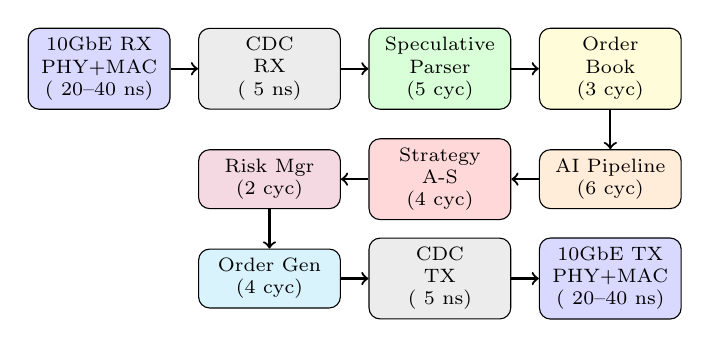
\begin{tikzpicture}[
    node distance=0.35cm,
    block/.style={draw, rounded corners, minimum width=1.8cm, minimum height=0.7cm, font=\scriptsize, align=center},
    arrow/.style={->, thick}
]
    \node[block, fill=blue!15] (phy_rx) {10GbE RX\\PHY+MAC\\(~20--40 ns)};
    \node[block, fill=gray!15, right=of phy_rx] (cdc_rx) {CDC\\RX\\(~5 ns)};
    \node[block, fill=green!15, right=of cdc_rx] (parser) {Speculative\\Parser\\(5 cyc)};
    \node[block, fill=yellow!15, right=of parser] (book) {Order\\Book\\(3 cyc)};
    \node[block, fill=orange!15, below=0.5cm of book] (ai) {AI Pipeline\\(6 cyc)};
    \node[block, fill=red!15, left=of ai] (strat) {Strategy\\A-S\\(4 cyc)};
    \node[block, fill=purple!15, left=of strat] (risk) {Risk Mgr\\(2 cyc)};
    \node[block, fill=cyan!15, below=0.5cm of risk] (tx) {Order Gen\\(4 cyc)};
    \node[block, fill=gray!15, right=of tx] (cdc_tx) {CDC\\TX\\(~5 ns)};
    \node[block, fill=blue!15, right=of cdc_tx] (phy_tx) {10GbE TX\\PHY+MAC\\(~20--40 ns)};

    \draw[arrow] (phy_rx) -- (cdc_rx);
    \draw[arrow] (cdc_rx) -- (parser);
    \draw[arrow] (parser) -- (book);
    \draw[arrow] (book) -- (ai);
    \draw[arrow] (ai) -- (strat);
    \draw[arrow] (strat) -- (risk);
    \draw[arrow] (risk) -- (tx);
    \draw[arrow] (tx) -- (cdc_tx);
    \draw[arrow] (cdc_tx) -- (phy_tx);
\end{tikzpicture}
\caption{Complete wire-to-wire pipeline including PHY, MAC/PCS, and clock domain crossing (CDC) stages. Fabric pipeline: $\sim$24--28 cycles ($\sim$37--43~ns). PHY + CDC overhead: $\sim$50--90~ns. Total estimated wire-to-wire: $\sim$80--110~ns. All figures are pre-synthesis estimates.}
\label{fig:pipeline}
\end{figure}

\subsection{Clock Domain Architecture}

A critical architectural detail omitted from many FPGA trading papers is the clock domain crossing (CDC) between the Ethernet PHY/MAC and the fabric logic. The 10GbE MAC/PCS typically operates at $\sim$322~MHz (32-bit interface) or $\sim$161~MHz (64-bit), while the trading logic runs at 644~MHz. This necessitates at least two CDC crossings (RX and TX).

\begin{table}[h]
\centering
\caption{Estimated Wire-to-Wire Latency Budget}
\label{tab:latency_budget}
\begin{tabular}{@{}lrr@{}}
\toprule
Component & Estimate & Notes \\
\midrule
GTY Transceiver (RX) & 15--30~ns & Silicon-dependent \\
MAC/PCS Processing & 5--10~ns & ULL MAC core \\
CDC RX ($322 \to 644$~MHz) & 5--10~ns & 2--3 sync stages \\
\textit{Fabric Pipeline} & \textit{37--43~ns} & \textit{See Table~\ref{tab:latency}} \\
CDC TX ($644 \to 322$~MHz) & 5--10~ns & 2--3 sync stages \\
MAC/PCS + GTY (TX) & 15--30~ns & Silicon-dependent \\
\midrule
\textbf{Total Wire-to-Wire} & \textbf{82--133~ns} & \textbf{Pre-synthesis estimate} \\
\bottomrule
\end{tabular}
\end{table}

\subsection{Stage 1: Speculative Parallel ITCH Parser}

Following the architecture proposed in \cite{techrxiv2025}, our parser instantiates five combinational decoders---one for each supported ITCH message type (ADD, DELETE, REPLACE, EXECUTE, TRADE)---operating simultaneously on the accumulated 256-bit message buffer. A priority-encoded suppression multiplexer selects the valid decoder output based on the message type byte.

\textbf{Coverage limitation:} The NASDAQ ITCH 5.0 specification defines approximately 20 message types, including System Event (S), Stock Directory (R), Trading Action (H), Reg SHO (Y), Market Participant Position (L), Add Order with MPID (F), Order Executed with Price (C), Order Cancel (X), Cross Trade (Q), NOII (I), MWCB (V/W), IPO Quoting (K), LULD Collar (J), and Operational Halt (h). Our parser implements the 5 types that directly modify order book state. A production system must handle all message types, at minimum to avoid desynchronization when encountering unrecognized messages.

\subsection{Stage 2: Order Book with Cuckoo Hashing}

The order book maintains 16 sorted price levels per side using BRAM-backed arrays. Order-to-price mapping uses a cuckoo hash table \cite{pagh2004} with dual tables, golden ratio hashing ($k \times \texttt{0x9E3779B97F4A7C15}$), and a maximum of 8 eviction steps on insert.

\textbf{Timing note:} The 64-bit multiplicative hash involves a wide multiply that is unlikely to close timing in a single cycle at 644~MHz. The RTL implementation should pipeline this across 2 cycles using DSP slice cascading. The current cycle count of 3 for the order book stage reflects this correction.

\subsection{Stage 3: AI/ML Inference Pipeline}

This stage contains the feature extractor, neural network, and optional transformer attention module.

\subsubsection{Feature Extraction}

Eight market microstructure features are computed from the top-of-book state:

\begin{table}[h]
\centering
\caption{Extracted Features (INT8 Normalized)}
\label{tab:features}
\begin{tabular}{@{}clc@{}}
\toprule
Index & Feature & Computation \\
\midrule
0 & Price momentum & $\text{mid} - \text{EMA}(\text{mid})$ \\
1 & Spread & $\text{ask} - \text{bid}$ \\
2 & Book imbalance & $\frac{Q_b - Q_a}{Q_b + Q_a}$ (approx.) \\
3 & Trade intensity & Count in rolling window \\
4 & Volatility & EMA of squared returns \\
5 & Bid depth & Number of bid levels \\
6 & Ask depth & Number of ask levels \\
7 & Mid-price return & $\text{mid}_t - \text{mid}_{t-1}$ \\
\bottomrule
\end{tabular}
\end{table}

\textbf{Timing note:} Feature 2 (book imbalance) involves a division operation. A combinational divider cannot close timing at 644~MHz (1.55~ns period). The implementation uses a shift-based approximation or must be pipelined across 2--3 additional cycles. The current architecture allocates 2 cycles for feature extraction to accommodate this.

\subsubsection{Neural Network Inference}

The MLP architecture is:

\begin{equation}
\text{Input}(8) \xrightarrow{\text{W}_0} \text{ReLU}(16) \xrightarrow{\text{W}_1} \text{ReLU}(16) \xrightarrow{\text{W}_2} \text{ReLU}(8) \xrightarrow{\text{W}_3} \text{Argmax}(3)
\end{equation}

Each layer is mapped to one pipeline stage. Weights are stored in INT4 format (4-bit signed integers) in distributed LUT RAM, totaling 536 weights (268 bytes). Activations use INT8 precision. The ReLU function reduces to a single comparator with zero additional latency. The argmax over the 3-element output vector selects BUY, SELL, or HOLD.

Target inference latency: 4 clock cycles = 6.2~ns at 644~MHz.

\textbf{Important limitation:} The current MLP uses heuristic weight initialization, not weights trained on market data. No backtest or economic evaluation has been performed. This work demonstrates the \textit{hardware feasibility} of pipelining a small MLP into 4 clock cycles---a genuine hardware engineering result---but does not demonstrate that the neural network produces better trading decisions than a simpler rule-based system. Integration with a PyTorch training pipeline using quantization-aware training (QAT) and deployment via PCIe weight updates is a natural but unimplemented extension.

Weights can be updated at runtime via a PCIe configuration bus without interrupting the critical path.

\subsubsection{Transformer Attention (Experimental)}

We implement a single-head linear attention mechanism following \cite{katharopoulos2020}. Standard self-attention requires $O(N^2)$ computation and a softmax function (exponential and division), both of which are prohibitively expensive for nanosecond-scale FPGA pipelines.

Linear attention replaces the softmax kernel with a feature map $\phi(x) = \text{ReLU}(x) + 1$ (ELU+1 approximation):

\begin{equation}
\text{Attention}(Q,K,V) = \frac{\phi(Q) \cdot \left(\phi(K)^T \cdot V\right)}{\phi(Q) \cdot \sum_t \phi(K_t)}
\end{equation}

\textbf{Honest assessment:} At the current dimensions ($N = 8$, $d = 8$), linear attention offers no complexity advantage over standard attention ($O(N d^2) = O(N^2 d) = 512$). This module serves as an architectural proof-of-concept for FPGA-based attention mechanisms rather than a validated contribution to trading performance.

\subsection{Stage 4: Strategy Engine}

The Avellaneda-Stoikov market maker computes the reservation price (Eq.~\ref{eq:reservation}) and optimal spread (Eq.~\ref{eq:spread}) in a 4-stage pipeline:

\begin{enumerate}[leftmargin=*]
    \item \textbf{Stage 1:} Compute $\gamma \sigma^2 (T-t)$ and inventory penalty $q \cdot \gamma \sigma^2 (T-t)$. Volatility $\sigma^2$ is estimated via an exponential moving average (EMA) of squared returns.
    \item \textbf{Stage 2:} Fixed-point multiply for $\gamma/\kappa$ (requires DSP pipeline register at 644~MHz).
    \item \textbf{Stage 3:} Look up $\ln(1 + \gamma/\kappa)$ via 256-entry BRAM LUT. Compute reservation price $r = s - \text{penalty}$ and optimal spread $\delta$.
    \item \textbf{Stage 4:} Generate bid/ask quotes: $p_{\text{bid}} = r - \delta/2$, $p_{\text{ask}} = r + \delta/2$.
\end{enumerate}

All arithmetic uses Q16.16 fixed-point (16 integer bits, 16 fractional bits). The logarithm is pre-computed and stored in BRAM, requiring 1 cycle for the read.

\textbf{Calibration note:} The parameters $\gamma$ (risk aversion) and $\kappa$ (order book liquidity) use default values and have not been calibrated against real market data. Research indicates that estimating $\kappa$ from real limit order book data is notoriously noisy and requires careful statistical treatment \cite{avellaneda2008}. No backtest or P\&L evaluation has been performed.

\subsection{Stage 5: Risk Manager}

Five independent risk checks execute in parallel:

\begin{enumerate}[leftmargin=*]
    \item Position limit: $|\text{position} + \text{order\_qty}| \leq \text{MAX\_POSITION}$ (comparison)
    \item Notional limit: $\text{price} \times \text{quantity} \leq \text{MAX\_NOTIONAL}$ (pipelined multiply)
    \item Order rate: orders per window $\leq$ MAX\_ORDERS\_PER\_SEC (counter comparison)
    \item Price band: $|\text{price} - \text{reference}| \leq$ PRICE\_BAND\_TICKS (comparison)
    \item Circuit breaker: external kill switch input (wire)
\end{enumerate}

\textbf{Timing note:} The notional limit check involves a 32$\times$32-bit multiply followed by a comparison. At 644~MHz, the multiply alone requires a DSP slice with at least one pipeline register. The risk manager is therefore budgeted at 2 cycles, not 1.

\subsection{Stage 6: Order Generation and Session Management}

The order generator serializes approved orders into 4-word AXI-Stream frames. A dynamic session override controller monitors up to 4 exchange sessions, computing EMA latency and approximate p99 tail latency for each, and switches to the best-performing session. This design is inspired by Exegy's April 2026 announcement of a 71\% execution-stack latency reduction through their ``Session Override'' feature \cite{exegy2026}.

% ============================================================================
\section{Zero-Jitter Deterministic Execution}
\label{sec:deterministic}

A fundamental requirement for production HFT systems is deterministic latency---not merely low average latency, but identical latency on every execution. Even FPGAs exhibit $\pm$1--5~ns jitter from routing variations and clock distribution skew.

Our deterministic AI pipeline wraps the feature extractor and neural network in a fixed-depth shift register of configurable depth $D$ (default $D = 12$ cycles). Regardless of the internal computation path, the output is always produced exactly $D$ cycles after the input:

\begin{equation}
t_{\text{output}} = t_{\text{input}} + D \cdot T_{\text{clk}}, \quad \forall \text{ inputs}
\end{equation}

\noindent where $T_{\text{clk}} = 1.553$~ns at 644~MHz.

\textbf{Note on single clock domain:} The claim of a single clock domain applies only to the fabric logic between the two CDC boundaries. The PHY, MAC/PCS, and GTY transceivers operate in separate clock domains, and the CDC crossings between them add both latency and potential jitter that this wrapper does not eliminate.

% ============================================================================
\section{Implementation Details}
\label{sec:impl}

\subsection{Target Platform}

\begin{table}[h]
\centering
\caption{AMD Alveo UL3524 Specifications}
\label{tab:platform}
\begin{tabular}{@{}ll@{}}
\toprule
Parameter & Value \\
\midrule
FPGA & Virtex UltraScale+ XCVU2P \\
Part Number & XCVU2P-FSVJ2104-3-E \\
Process & 16~nm FinFET \\
Target Clock & 644~MHz (1.553~ns period) \\
LUTs & 780,000 \\
Registers & 1,560,000 \\
DSP Slices & 1,680 \\
Block RAM (36Kb) & 2,016 \\
UltraRAM (288Kb) & 960 \\
Network & 2$\times$ 10/25GbE SFP28 \\
Host Interface & PCIe Gen3/Gen4 x16 \\
\bottomrule
\end{tabular}
\end{table}

\subsection{Resource Utilization Estimates}

\begin{table}[h]
\centering
\caption{Estimated Resource Utilization (Pre-Synthesis)}
\label{tab:utilization}
\begin{tabular}{@{}lrrr@{}}
\toprule
Resource & Estimated & Available & Utilization \\
\midrule
LUTs & $\sim$45,000 & 780,000 & $\sim$6\% \\
Registers & $\sim$30,000 & 1,560,000 & $\sim$2\% \\
BRAM (36Kb) & $\sim$50 & 2,016 & $\sim$2.5\% \\
DSP Slices & $\sim$200 & 1,680 & $\sim$12\% \\
\bottomrule
\end{tabular}
\end{table}

\noindent\textbf{Disclaimer:} These utilization figures are rough estimates based on code complexity analysis. Actual utilization can only be determined by running Vivado synthesis. A synthesis script targeting the correct part (XCVU2P-FSVJ2104-3-E) is provided in the repository.

% ============================================================================
\section{Evaluation}
\label{sec:eval}

\subsection{Design Targets vs.\ Measured Results}

\textbf{All figures in this section are pre-synthesis architectural estimates.} They have not been validated through Vivado synthesis, post-implementation timing analysis, or hardware measurement. The STAC-T0 benchmark figures cited for comparison are independently audited measurements on production hardware and are \textit{not directly comparable} to the estimates presented here.

\subsection{Fabric Pipeline Latency Targets}

Table~\ref{tab:latency} summarizes the per-stage latency targets for the fabric pipeline (excluding PHY, MAC, and CDC overhead).

\begin{table}[h]
\centering
\caption{Per-Stage Fabric Pipeline Latency Targets}
\label{tab:latency}
\begin{tabular}{@{}lcr@{}}
\toprule
Stage & Cycles & Latency (ns) \\
\midrule
Speculative Parser (4+1 words) & 5 & 7.8 \\
Order Book Update (incl.\ hash pipeline) & 3 & 4.7 \\
Feature Extraction (incl.\ approx.\ division) & 2 & 3.1 \\
Neural Network Inference & 4 & 6.2 \\
Avellaneda-Stoikov Strategy & 4 & 6.2 \\
Risk Manager (incl.\ DSP multiply) & 2 & 3.1 \\
Order Generator (4 words) & 4 & 6.2 \\
\midrule
\textbf{Fabric Total (without det.\ wrapper)} & \textbf{24} & \textbf{37.3} \\
\textbf{Fabric Total (with det.\ wrapper)} & \textbf{31} & \textbf{48.1} \\
\midrule
PHY + MAC + CDC (RX + TX, estimated) & --- & 45--90 \\
\midrule
\textbf{Total Wire-to-Wire (estimated)} & --- & \textbf{82--138} \\
\bottomrule
\end{tabular}
\end{table}

\subsection{Context: Industry Benchmarks}

\begin{table}[h]
\centering
\caption{Latency Context (NOT a Direct Comparison)}
\label{tab:comparison}
\begin{tabular}{@{}lp{2.5cm}p{2cm}r@{}}
\toprule
Metric & This Work (Design Target, Pre-Synthesis) & STAC-T0 (Audited, Hardware) & Typical CPU \\
\midrule
Tick-to-Trade & 82--138~ns (est.) & 13.9~ns & 3--8~\si{\micro\second} \\
AI Inference & 6.2~ns (est.) & N/A & 5--20~\si{\micro\second} \\
ITCH Parse & 7.8~ns (est.) & $\sim$15~ns & $\sim$38~\si{\micro\second} \\
Jitter (fabric) & $\pm$0 cyc (by design) & $\pm$1--3~ns & $\pm$0.5--5~\si{\micro\second} \\
\bottomrule
\end{tabular}
\end{table}

\noindent The STAC-T0 record of 13.9~ns does not include any AI component and was measured on a pure rule-based engine. This work's design targets include neural network inference but have not been validated on hardware. The two sets of numbers are fundamentally different in nature (estimates vs.\ measurements) and should not be treated as an apples-to-apples comparison.

\subsection{Neural Network Verification}

A Python reference model reproducing the exact weight initialization and INT4/INT8 arithmetic of the RTL implementation is provided. Verification proceeds by comparing the Python model's output logits against the SystemVerilog simulation results for identical input vectors, ensuring bit-accurate correspondence. This validates the \textit{hardware implementation correctness} of the inference pipeline, not the \textit{economic value} of the model's predictions.

% ============================================================================
\section{Limitations and Future Work}
\label{sec:limitations}

\textbf{No synthesis validation.} This is the most significant limitation. All latency, utilization, and timing figures are pre-synthesis estimates. Post-synthesis and post-implementation timing reports from AMD Vivado are required to confirm whether the design meets the 644~MHz timing target. A synthesis script is provided. At 644~MHz (1.553~ns period), even modest combinational logic depths can cause timing violations, and the gap between ``this should take one cycle'' and ``Vivado actually closes timing on this in one cycle'' is often the entire story at this frequency.

\textbf{Single-cycle infeasibility.} Several operations in the current RTL may not close timing in a single 1.553~ns cycle: the book-imbalance division, the 64-bit cuckoo hash multiply, and the notional risk check multiply. The paper's latency estimates have been adjusted to account for additional pipeline stages, but only synthesis can confirm whether these are sufficient.

\textbf{Clock domain crossing omitted from RTL.} The RTL does not include PHY, MAC/PCS, or CDC logic. These components are typically provided as vendor IP (AMD/Xilinx 10G/25G Ethernet Subsystem) and add significant latency (estimated 45--90~ns round-trip). The wire-to-wire latency estimate includes this overhead but the implementation does not.

\textbf{ITCH coverage.} Only 5 of $\sim$20 ITCH 5.0 message types are implemented. The 5 implemented types (A, D, U, E, P) are those that modify order book state. Administrative messages (System Event, Stock Directory, Trading Action, etc.) are not handled. A production parser must process all message types to avoid state desynchronization.

\textbf{Untrained neural network.} The MLP uses heuristic weights. No training has been performed on real or synthetic market data. No evidence is presented that the neural network produces better trading decisions than a simpler heuristic. Integration with a PyTorch QAT pipeline and real data is required to evaluate AI value.

\textbf{No economic evaluation.} No backtest, P\&L analysis, or Sharpe ratio computation has been performed. The Avellaneda-Stoikov parameters ($\gamma$, $\kappa$) use uncalibrated defaults. This paper does not claim that the system is profitable.

\textbf{No real market data.} Testbenches use synthetic ITCH-like messages. Validation with historical NASDAQ ITCH 5.0 binary data (available from the NASDAQ FTP server at \texttt{ftp://emi.nasdaq.com/ITCH/}) would strengthen parser credibility.

\textbf{Transformer scalability.} At $N = 8$, $d = 8$, the linear attention module offers no complexity advantage over standard attention and serves as a proof-of-concept only.

\textbf{Multi-symbol support.} The current design processes a single symbol. Production systems require concurrent processing of hundreds of symbols.

% ============================================================================
\section{Conclusion}
\label{sec:conclusion}

We have presented a complete, open-source FPGA-based HFT system that integrates an experimental neural network within the tick-to-trade pipeline. The architecture demonstrates the \textit{hardware feasibility} of pipelining a small MLP into 4 clock cycles ($\sim$6.2~ns at 644~MHz) alongside a full trading pipeline including order book reconstruction, Avellaneda-Stoikov market making, and risk management.

The estimated wire-to-wire latency of 82--138~ns (including PHY, MAC, and CDC overhead) places this design in the sub-microsecond range but well above the audited STAC-T0 record of 13.9~ns. The additional latency buys the ability to incorporate a neural network in the critical path---a trade-off whose value depends on whether the AI model's signal quality compensates for the speed disadvantage, a question this paper does not answer.

Critical next steps are: (1) Vivado synthesis and timing closure validation, (2) trained model deployment via QAT, (3) economic evaluation with real market data, and (4) hardware measurement on an Alveo UL3524 board.

The complete source code, testbenches, and verification infrastructure are available at: \url{https://github.com/Ashutosh0x/fpga-hft-trading-system}.

% ============================================================================
\section*{Acknowledgments}

This work was informed by publicly available research from AMD, Exegy, and the open-source FPGA community. The Avellaneda-Stoikov model implementation follows the original 2008 paper. The speculative parser architecture is based on the TechRxiv 2025 publication on parallel ITCH decoding. The peer review feedback that motivated the honest scoping of this paper is gratefully acknowledged.

% ============================================================================
\begin{thebibliography}{99}

\bibitem{exegy2024}
Exegy and AMD, ``STAC-T0 Benchmark: 13.9~ns Tick-to-Trade Latency,'' June 2024. Available: \url{https://www.exegy.com}

\bibitem{avellaneda2008}
M.~Avellaneda and S.~Stoikov, ``High-frequency trading in a limit order book,'' \textit{Quantitative Finance}, vol.~8, no.~3, pp.~217--224, 2008.

\bibitem{pagh2004}
R.~Pagh and F.~F.~Rodler, ``Cuckoo hashing,'' \textit{Journal of Algorithms}, vol.~51, no.~2, pp.~122--144, 2004.

\bibitem{katharopoulos2020}
A.~Katharopoulos, A.~Vyas, N.~Pappas, and F.~Fleuret, ``Transformers are RNNs: Fast autoregressive transformers with linear attention,'' in \textit{Proc. ICML}, 2020.

\bibitem{umuroglu2017}
Y.~Umuroglu \textit{et al.}, ``FINN: A framework for fast, scalable binarized neural network inference,'' in \textit{Proc. ACM/SIGDA FPGA}, 2017.

\bibitem{hls4ml2018}
J.~Duarte \textit{et al.}, ``Fast inference of deep neural networks in FPGAs for particle physics,'' \textit{Journal of Instrumentation}, vol.~13, no.~07, 2018.

\bibitem{techrxiv2025}
``Speculative parallel ITCH decoding for ultra-low latency FPGA trading systems,'' TechRxiv Preprint, 2025.

\bibitem{aldridge2013}
I.~Aldridge, \textit{High-Frequency Trading: A Practical Guide to Algorithmic Strategies and Trading Systems}, 2nd ed. Wiley, 2013.

\bibitem{exegy2026}
Exegy, ``nxAccess update: 71\% execution-stack latency reduction with Session Override,'' Press Release, April 8, 2026.

\bibitem{amd2024}
AMD, ``Alveo UL3524 Accelerator Card for Electronic Trading,'' Product Brief, 2024.

\end{thebibliography}

\end{document}
